\documentclass{article}
\usepackage[utf8]{inputenc}
\usepackage{graphicx}
\usepackage[table,xcdraw]{xcolor}
\usepackage{geometry}
\geometry{a4paper, margin=1in}
\usepackage{float}
\usepackage{hyperref}

\title{COMPSCI 589 - Final Project: Spring 2026}
\author{Marwan Hegab \and Peter Ye \and Max Goldman}
\date{\today}

\begin{document}

\maketitle

\section*{Extra Credit Declarations}
\textcolor{red}{\textbf{[Extra Credit Question \#1] (10 Points):}} We analyzed all four datasets using an additional algorithm. For Dataset 1, we evaluated three algorithms (k-NN, Random Forest, and Neural Networks) rather than the required two.

\noindent\textcolor{red}{\textbf{[Extra Credit Question \#2] (10 Points):}} For an extra, challenging dataset, we used a modified version of the GTZAN Music Genre dataset (can be found \href{https://www.kaggle.com/datasets/andradaolteanu/gtzan-dataset-music-genre-classification}{here}).
This dataset has 58 attributes that characterize the waveform and musical qualities of a song, and the label is assigned as one of 10 genres. 
It has 1000 instances total, 100 for each genre, and has a modification to add a categorical attribute that describes the tempo of the song using Italian tempo marking (e.g. Allegro, Andante).

\noindent\textcolor{red}{\textbf{[Extra Credit Question \#3] (15 Points):}} We created a hybrid ensemble composed of equal parts bootstrapped kNNs and Decision Trees, and evaluated it on the Rice Grains dataset with varying tree/kNN values.

\section{Experiments and Analyses}

\subsection{Dataset 1: The Hand-Written Digits Recognition Dataset}

\textbf{Task Assigned To:} Marwan Hegab. \\
\textbf{Implementations Used:} Peter's implementation of k-NN, Max's implementation of Random Forest, and Marwan's implementation of Neural Networks.

\textbf{Algorithm Selection Rationale:} k-NN and Neural Networks were primary choices for this dataset because they traditionally preform relatively well at image recognition and capturing relationships in pixel data. Additionally, Random Forest serves as a strong, non-linear ensemble baseline to compare against.

- Each instance of the dataset represents an $8 \times 8$ grayscale image resulting in 64 numerical attributes. We globally normalized all pixel intensities by dividing them by 16.0 (the maximum pixel value) prior to training to ensure scale consistency across all three algorithms.

- The performance of each of the three algorithms was evaluated using Stratified 10-Fold Cross-Validation, measuring both Accuracy and F1-Score (Weighted). 

\subsubsection{Hyperparameter Tuning}

At least 6 different hyperparameter settings were used for each algorithm. The results averaged across the 10 folds are shown below:

\textbf{1. k-Nearest Neighbors (k-NN):}
\begin{table}[H]
\centering
\begin{tabular}{|l|c|c|}
\hline
\textbf{Hyperparameter ($k$)} & \textbf{Accuracy} & \textbf{F1-Score} \\ \hline
$k = 1$ & \textbf{0.9894} & \textbf{0.9894} \\ \hline
$k = 3$ & 0.9894 & 0.9893 \\ \hline
$k = 5$ & 0.9861 & 0.9860 \\ \hline
$k = 7$ & 0.9861 & 0.9861 \\ \hline
$k = 9$ & 0.9833 & 0.9833 \\ \hline
$k = 15$ & 0.9805 & 0.9805 \\ \hline
\end{tabular}
\end{table}
\noindent The optimal hyperparameter for k-NN is $k=1$.

\textbf{2. Random Forest:}
\begin{table}[H]
\centering
\begin{tabular}{|l|c|c|}
\hline
\textbf{Hyperparameter (\# of Trees)} & \textbf{Accuracy} & \textbf{F1-Score} \\ \hline
$trees = 1$ & 0.8046 & 0.8036 \\ \hline
$trees = 5$ & 0.9305 & 0.9302 \\ \hline
$trees = 10$ & 0.9555 & 0.9556 \\ \hline
$trees = 15$ & 0.9616 & 0.9616 \\ \hline
$trees = 20$ & 0.9694 & 0.9695 \\ \hline
$trees = 30$ & \textbf{0.9722} & \textbf{0.9721} \\ \hline
\end{tabular}
\end{table}
\noindent The optimal hyperparameter for Random Forest is $trees=30$.

\textbf{3. Neural Network (Base: Epochs=250, Batch=32):}
\begin{table}[H]
\centering
\resizebox{\textwidth}{!}{%
\begin{tabular}{|l|c|c|}
\hline
\textbf{Hyperparameters (Architecture, Alpha, Lambda)} & \textbf{Accuracy} & \textbf{F1-Score} \\ \hline
Arch=[32, 10], $\alpha=0.1$, $\lambda=0.01$ (Baseline) & 0.9755 & 0.9755 \\ \hline
Arch=[16, 10], $\alpha=0.1$, $\lambda=0.01$ (Shallower) & 0.9694 & 0.9693 \\ \hline
Arch=[64, 32, 10], $\alpha=0.1$, $\lambda=0.01$ (Deeper) & 0.9772 & 0.9772 \\ \hline
Arch=[32, 10], $\alpha=0.01$, $\lambda=0.01$ (Low LR) & 0.9360 & 0.9356 \\ \hline
Arch=[32, 10], $\alpha=0.5$, $\lambda=0.01$ (High LR) & \textbf{0.9816} & \textbf{0.9816} \\ \hline
Arch=[32, 10], $\alpha=0.1$, $\lambda=0.1$ (High Reg) & 0.9549 & 0.9550 \\ \hline
\end{tabular}%
}
\end{table}
\noindent The optimal hyperparameters for the Neural Network are Architecture=[32, 10], $\alpha=0.5$, and $\lambda=0.01$.

\subsubsection{Learning Curves and Analysis}

Below are the learning curves for the three evaluated algorithms.

\begin{figure}[H]
    \centering
    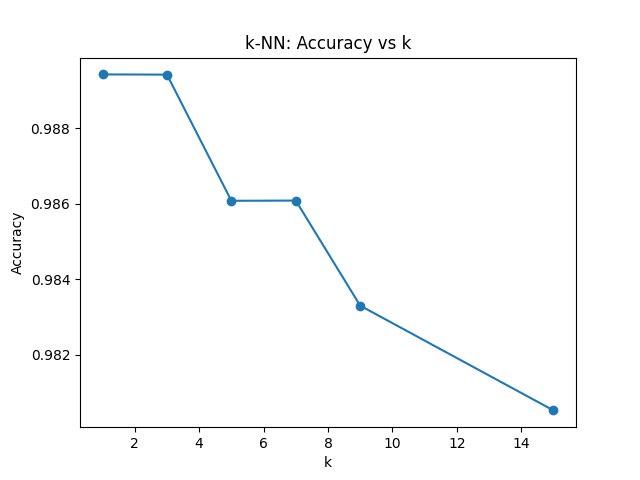
\includegraphics[width=0.6\textwidth]{figures/dataset1_knn_acc.png}
    \caption{k-NN Learning Curve: Accuracy vs. $k$}
\end{figure}

\begin{figure}[H]
    \centering
    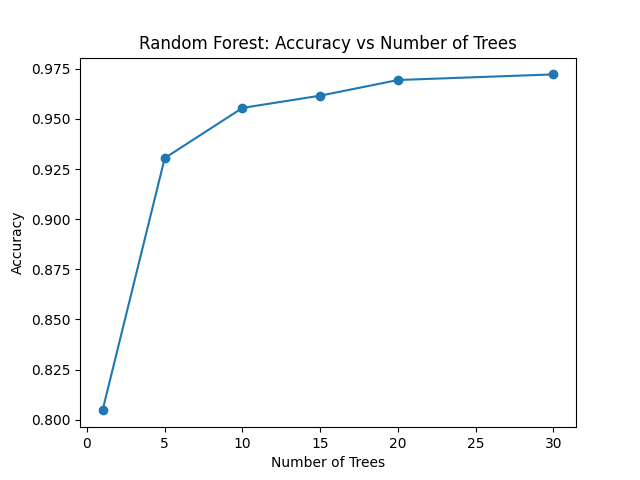
\includegraphics[width=0.6\textwidth]{figures/dataset1_rf_acc.png}
    \caption{Random Forest Learning Curve: Accuracy vs. Number of Trees}
\end{figure}

\begin{figure}[H]
    \centering
    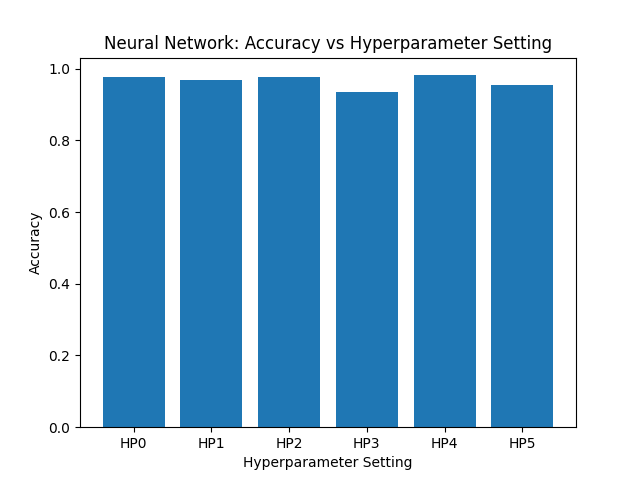
\includegraphics[width=0.6\textwidth]{figures/dataset1_nn_acc.png}
    \caption{Neural Network Bar Chart: Accuracy vs. Hyperparameter Setting}
\end{figure}

\begin{figure}[H]
    \centering
    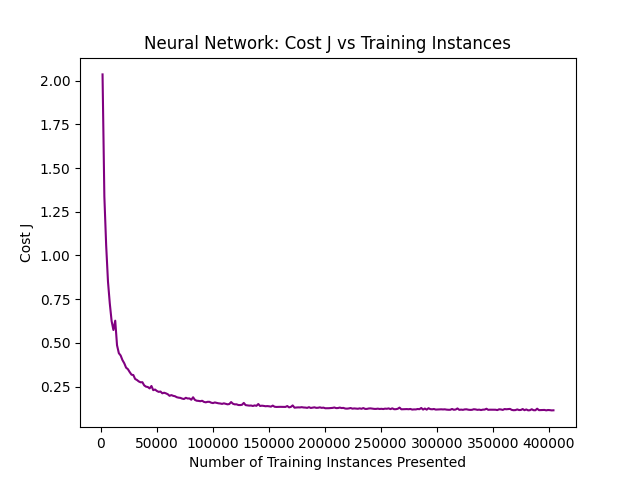
\includegraphics[width=0.6\textwidth]{figures/dataset1_nn_cost.png}
    \caption{Neural Network Learning Curve: Cost $J$ vs. Training Instances Presented}
\end{figure}

\textbf{Analysis and Interpretation:}
- The k-NN algorithm achieved the highest overall performance on Dataset 1 with an accuracy of $98.94\%$. In the domain of handwritten digit recognition, image samples of the exact same digit map very closely to each other in Euclidean space because their dark pixels heavily overlap. This results in tight, highly predictive spatial clusters, making k-NN heavily effective, specifically when $k$ is small ($k=1$ or $k=3$).

- The Random Forest's performance steadily improved as the number of trees grew to 30, capturing the non-linear relationships between individual pixel intensities and the 10 target classes. The Neural Network performed best with a higher learning rate ($\alpha=0.5$), suggesting that the digit classification task has a relatively smooth loss landscape that benefits from larger gradient steps. Smaller learning rates (e.g., $\alpha=0.01$) converged too slowly within the fixed 250 epochs, while stronger regularization ($\lambda=0.1$) slightly over-constrained the weights, reducing expressiveness on a 10-class problem.




\newpage




\subsection{Dataset 4: The Credit Approval Dataset}

\textbf{Task Assigned To:} Max Goldman \\
\textbf{Implementations Used:} Max's implementation of Decision Tree and Random Forest, Marwan's implementation of Neural Network.

\noindent\textbf{Algorithm Selection Rationale:}
The decision tree algorithm was selected since the human credit approval process is intuitively similar, and the model should be able to learn the patterns well.
The random forest was selected to compare with the decision tree, since it is aimed to aid the problem of overfitting that commonly arises, but it still follows the same intuitive model.
The neural network was selected since it can capture more complex nonlinear relationships in the data, and it will provide a good comparison for non-decision-based models.

\subsubsection{Hyperparameter Tuning}

6 different hyperparameter settings were used for each algorithm. The performance of each of the three algorithms was evaluated using Stratified 10-Fold Cross-Validation, measuring both Accuracy and F1-Score (Weighted). 
The results averaged across the 10 folds are shown below:

\vspace{0.25cm}

\textbf{1. Decision Tree:}
\begin{table}[H]
\centering
\begin{tabular}{|l|c|c|}
\hline
\textbf{Hyperparameter ($max\_depth$)} & \textbf{Accuracy} & \textbf{F1-Score} \\ \hline
$max\_depth = 1$ & \textbf{0.8637} & \textbf{0.8636} \\ \hline
$max\_depth = 3$ & 0.8591 & 0.8590 \\ \hline
$max\_depth = 5$ & 0.8284 & 0.8276 \\ \hline
$max\_depth = 7$ & 0.8224 & 0.8214 \\ \hline
$max\_depth = 9$ & 0.8163 & 0.8155 \\ \hline
$kmax\_depth = 15$ & 0.8209 & 0.8202 \\ \hline
\end{tabular}
\end{table}
\noindent The optimal hyperparameter for the decision tree on this dataset is $max\_depth = 1$.
\vspace{0.25cm}

\textbf{2. Random Forest:}
\begin{table}[H]
\centering
\begin{tabular}{|l|c|c|}
\hline
\textbf{Hyperparameter (\# of Trees)} & \textbf{Accuracy} & \textbf{F1-Score} \\ \hline
$trees = 1$ & 0.7825 & 0.7821 \\ \hline
$trees = 5$ & 0.8377 & 0.8375 \\ \hline
$trees = 10$ & 0.8407 & 0.8404 \\ \hline
$trees = 20$ & 0.8576 & 0.8573 \\ \hline
$trees = 30$ & \textbf{0.8591} & \textbf{0.8591} \\ \hline
$trees = 40$ & 0.8514 & 0.8512 \\ \hline
\end{tabular}
\end{table}
\noindent The optimal hyperparameter for a Random Forest on this dataset is $trees=30$.
\vspace{0.25cm}

\textbf{3. Neural Network (Architecture: [10, 2], Alpha: 0.1, Lambda: 0.01):}
\begin{table}[H]
\centering
\begin{tabular}{|l|c|c|}
\hline
\textbf{Hyperparameter (Epochs)} & \textbf{Accuracy} & \textbf{F1-Score} \\ \hline
$epochs = 10$ & 0.8131 & 0.8114 \\ \hline
$epochs = 25$ & 0.8483 & 0.8481 \\ \hline
$epochs = 50$ & \textbf{0.8652} & \textbf{0.8652} \\ \hline
$epochs = 100$ & 0.8591 & 0.8593 \\ \hline
$epochs = 150$ & 0.8591 & 0.8592 \\ \hline
$epochs = 250$ & 0.8576 & 0.8577 \\ \hline
\end{tabular}
\end{table}
\noindent The optimal hyperparameter for the Neural Network is $epochs=50$.



\newpage
\subsubsection{Learning Curves and Analysis}

Below are the learning curves for the three evaluated algorithms.

\begin{figure}[H]
    \centering
    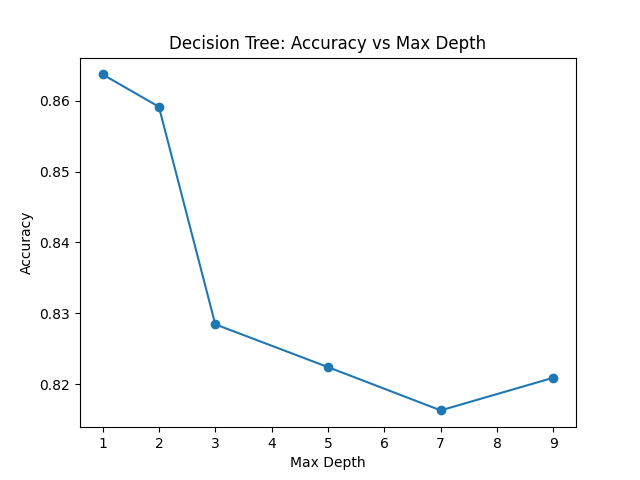
\includegraphics[width=0.6\textwidth]{figures/dataset4_dt_acc.png}
    \caption{Decision Tree Learning Curve: Accuracy vs. $max\_depth$}
\end{figure}

\begin{figure}[H]
    \centering
    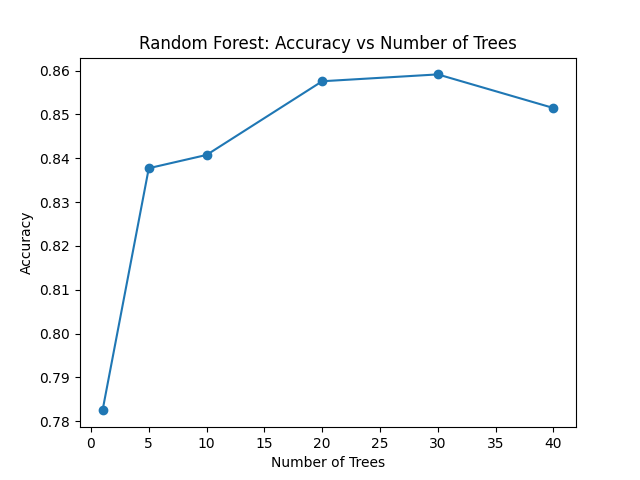
\includegraphics[width=0.6\textwidth]{figures/dataset4_rf_acc.png}
    \caption{Random Forest Learning Curve: Accuracy vs. Number of Trees}
\end{figure}

\begin{figure}[H]
    \centering
    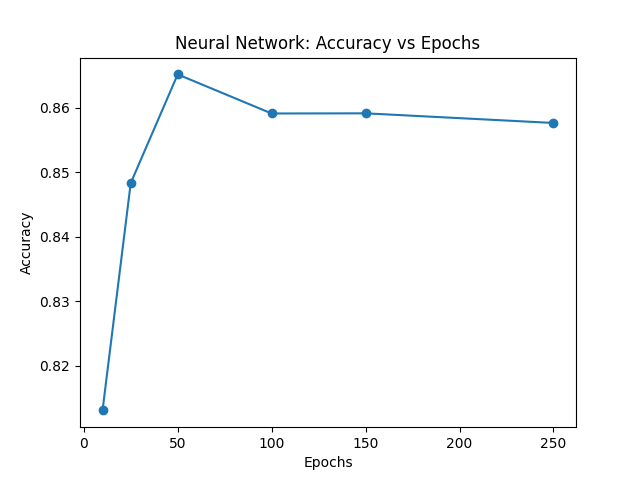
\includegraphics[width=0.6\textwidth]{figures/dataset4_nn_acc.png}
    \caption{Neural Network Learning Curve: Accuracy vs. Epochs}
\end{figure}

\begin{figure}[H]
    \centering
    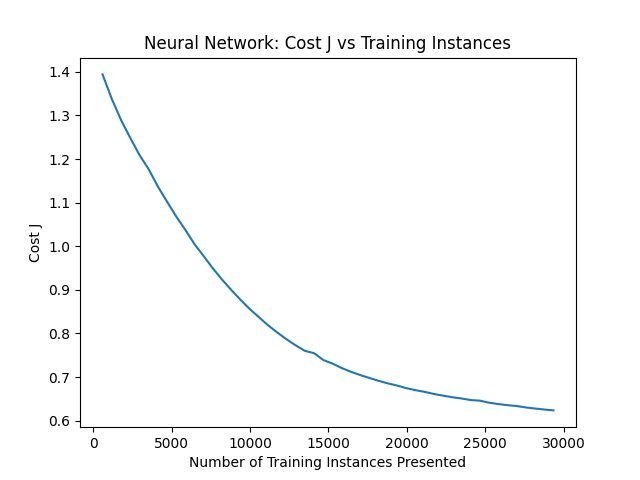
\includegraphics[width=0.6\textwidth]{figures/dataset4_nn_cost.png}
    \caption{Neural Network Learning Curve: Cost $J$ vs. Training Instances Presented}
\end{figure}

\noindent \textbf{Analysis and Interpretation:}

\noindent Overall, all 3 models performed fairly well, with optimized accuracies landing around $86\%$.
Surprisingly, the decision tree had its best performance with $max\_depth = 1$. 
This signals that there is one attribute that corresponds to the label $86\%$ of the time, and that further splitting of the data does not yield more accuracy.
Indeed, we can print this attribute during execution to reveal that \verb|attr9_cat| is "t" most of the time the label is 1, and "f" most of the time the label is 0.

This single decision performs so well, that a random forest cannot catch up. We saw a peak accuracy of $85.91\%$ at 30 trees, which fell short of $86.37\%$ in the 1 decision tree.
Perhaps if we ran some higher values of \verb|n_tree|, it may surpass, but 40 trees was already taking a long time to run so we omitted higher values from our analysis.

However, the neural network just barely ended up having the best performance with an accuracy of $86.52\%$. 
This is due to the fact that there are likely more complex nonlinear relationships within the data, since credit approval hinges on many interlinked factors
like income, debt, credit history, etc. The neural net was able to learn these relationships better than the degree of the single \verb|attr9_cat| decision.

Overall all 3 models perfomed very comparably. However, we can see from the cost function that we did not quite minimize our error on the neural net, so there is further optimization we could squeeze from this model.


\newpage




\subsection{\textcolor{red}{\textbf{[Extra Credit]}} Dataset 5: The Modified GTZAN Music Genre Dataset}

\textbf{Task Assigned To:} Max Goldman \\
\textbf{Implementations Used:} Max's implementation of Decision Tree and Random Forest, Marwan's implementation of Neural Network.

\noindent\textbf{About the Dataset:} The GTZAN Music Genre dataset classifies genres of music based on a collection of 58 numerical attributes related to the audio of the song. 
There are 10 genres with 100 instances each, adding up to 1000 instances total. 
In order to satisfy the "complex dataset" requirement, one attribute, bpm, was modified to create a categorical attribute, tempo, which holds the Italian tempo marking of the given audio (read about it \href{https://www.musicca.com/musical-terms}{here}).

\noindent\textbf{Algorithm Selection Rationale:}
The decision tree algorithm was selected since it has a similar intuition to how a human would classify a song. Attributes relating to the song could be categorized and classified, just like humans created genres.
The random forest was selected to compare with the decision tree, since it is aimed to aid the problem of overfitting that commonly arises, but it still follows the same intuitive model.
The neural network was selected since it can capture more complex nonlinear relationships in the data, and it will provide a good comparison for non-decision-based models.
It will likely perform the best since the data is mainly mathematical, spectral data relating to the audio files, and not really categorizing or qualitatively describing anything about the song.



\subsubsection{Hyperparameter Tuning}

6 different hyperparameter settings were used for each algorithm. The results averaged across the 10 folds are shown below:
- The performance of each of the three algorithms was evaluated using Stratified 10-Fold Cross-Validation, measuring both Accuracy and F1-Score (Weighted). 

\vspace{0.25cm}
\textbf{1. Decision Tree:}
\begin{table}[H]
\centering
\begin{tabular}{|l|c|c|}
\hline
\textbf{Hyperparameter ($tree\_depth$)} & \textbf{Accuracy} & \textbf{F1-Score} \\ \hline
$max\_depth = 2$ & 0.3080 & 0.1860 \\ \hline
$max\_depth = 4$ & 0.4510 & 0.4530 \\ \hline
$max\_depth = 6$ & 0.4660 & 0.4645 \\ \hline
$max\_depth = 8$ & 0.4980 & 0.4965 \\ \hline
$max\_depth = 10$ & \textbf{0.5020} & \textbf{0.4985} \\ \hline
$max\_depth = 12$ & 0.5020 & 0.4983 \\ \hline
\end{tabular}
\end{table}
\noindent The optimal hyperparameter for the decision tree on this dataset is $max\_depth = 10$.

\vspace{0.25cm}
\textbf{2. Random Forest:}
\begin{table}[H]
\centering
\begin{tabular}{|l|c|c|}
\hline
\textbf{Hyperparameter (\# of Trees)} & \textbf{Accuracy} & \textbf{F1-Score} \\ \hline
$trees = 1$ & 0.4420 & 0.4429 \\ \hline
$trees = 5$ & 0.5520 & 0.5438 \\ \hline
$trees = 10$ & 0.6130 & 0.6092 \\ \hline
$trees = 20$ & 0.6700 & 0.6681 \\ \hline
$trees = 30$ & 0.6980 & 0.6925 \\ \hline
$trees = 40$ & \textbf{0.7020} & \textbf{0.6957} \\ \hline
\end{tabular}
\end{table}
\noindent The optimal hyperparameter for a Random Forest on this dataset is $trees=30$.

\vspace{0.25cm}
\textbf{3. Neural Network (Architecture: [40, 40, 10], Alpha: 0.1, Lambda: 0.01):}
\begin{table}[H]
\centering
\begin{tabular}{|l|c|c|}
\hline
\textbf{Hyperparameter (Epochs)} & \textbf{Accuracy} & \textbf{F1-Score} \\ \hline
$epochs = 50$ & 0.6580 & 0.6471 \\ \hline
$epochs = 100$ & 0.7070 & 0.7020 \\ \hline
$epochs = 250$ & 0.7310 & 0.7269 \\ \hline
$epochs = 500$ & \textbf{0.7440} & \textbf{0.7410} \\ \hline
$epochs = 1000$ & 0.7380 & 0.7339 \\ \hline
$epochs = 2000$ & 0.7380 & 0.7342 \\ \hline
\end{tabular}
\end{table}
\noindent The optimal hyperparameter for the Neural Network is $epochs=500$.

\newpage

\subsubsection{Learning Curves and Analysis}

Below are the learning curves for the three evaluated algorithms.

\begin{figure}[H]
    \centering
    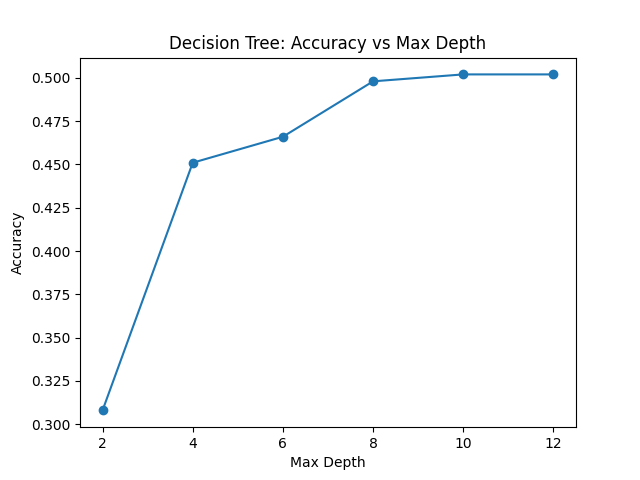
\includegraphics[width=0.6\textwidth]{figures/dataset5_dt_acc.png}
    \caption{Decision Tree Learning Curve: Accuracy vs. $max\_depth$}
\end{figure}

\begin{figure}[H]
    \centering
    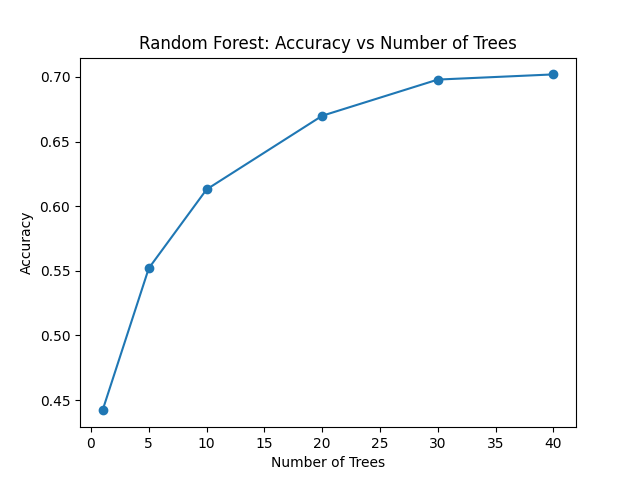
\includegraphics[width=0.6\textwidth]{figures/dataset5_rf_acc.png}
    \caption{Random Forest Learning Curve: Accuracy vs. Number of Trees}
\end{figure}

\begin{figure}[H]
    \centering
    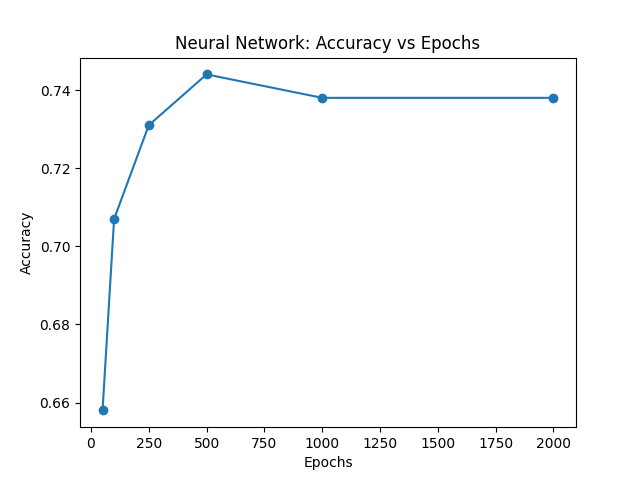
\includegraphics[width=0.6\textwidth]{figures/dataset5_nn_acc.png}
    \caption{Neural Network Learning Curve: Accuracy vs. Epochs}
\end{figure}

\begin{figure}[H]
    \centering
    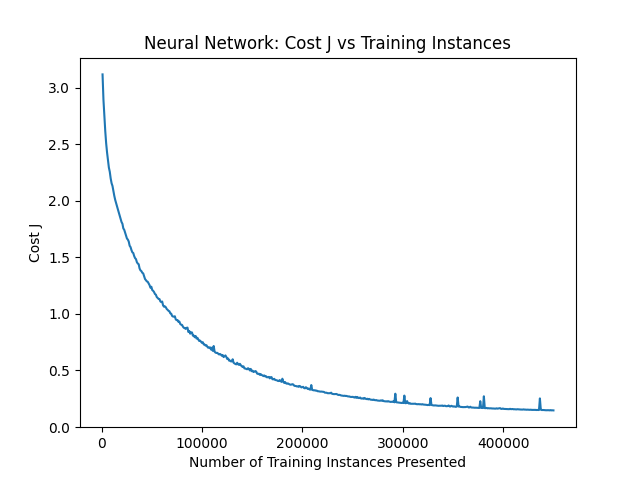
\includegraphics[width=0.6\textwidth]{figures/dataset5_nn_cost.png}
    \caption{Neural Network Learning Curve: Cost $J$ vs. Training Instances Presented}
\end{figure}

\textbf{Analysis and Interpretation:}
As expected, the neural network by far had the highest performance, with an optimized accuracy of $74.4\%$ at 500 epochs. 
We can see that we pushed the cost function pretty low with this configuration, so we can say it is relatively optimized.

On the other hand, our decision tree did not perform nearly as well, but still was able to make some decent progress with an optimized accuracy of $50.2\%$ at $max\_depth = 10$.
Considering there are 10 possible labels, a random guess would have an accuracy of $10\%$, so this is way better than random, but still not at the level of the neural net.

The random forest performed much better than the decision tree, with an optimized accuracy of $70.2\%$ at \verb|n_tree = 40|. 
Again, with a higher \verb|n_tree| value we may have been able to squeeze just a little bit more performance out of it, but the algorithm was already taking an extremely long time to train and we can see the accuracy plateau strongly already.

Overall though, the neural network had the best performance as it was able to learn the complex relationships in the mathematical data.

\newpage



\subsection{\textcolor{red}{\textbf{[Extra Credit]}} Hybrid kNN-Decision-Tree Ensemble}

\textbf{Task Assigned To:} Max Goldman \\
\textbf{Implementations Used:} Max's implementation of Decision Tree and Random Forest, Peter's implementation of kNN.

\noindent\textbf{Algorithm Explanation:}
This hybrid ensemble consists of equal parts kNN and decision tree. 
For each individual kNN "vote" in the ensemble, the kNN algorithm is run on a corresponding bootstrapped dataset.
Decision tree votes work the same as in a random forest. 
After every member of the ensemble has voted, either the majority wins, or a random choice is made if there is a tie.



\subsubsection{Hyperparameter Tuning}

The chosen hyperparameter for this ensemble is $n$, which represents the number of trees and the number of kNNs.
That is, there will be $n$ trees and $n$ kNNs evaluated, so there will be $2n$ votes total. 
The $k$ value for the kNNs is held at 3, and 6 different hyperparameter settings were used for each dataset. 
The performance of the algorithm was evaluated using Stratified 10-Fold Cross-Validation, measuring both Accuracy and F1-Score (Weighted).
The results averaged across the 10 folds are shown below: 

\vspace{0.25cm}
\textbf{1. Parkinson's Dataset:}
\begin{table}[H]
\centering
\begin{tabular}{|l|c|c|}
\hline
\textbf{Hyperparameter ($n$)} & \textbf{Accuracy} & \textbf{F1-Score} \\ \hline
$n = 1$ & 0.8045 & 0.7658 \\ \hline
$n = 3$ & 0.8408 & 0.8013 \\ \hline
$n = 5$ & \textbf{0.8816} & \textbf{0.8607} \\ \hline
$n = 7$ & 0.8255 & 0.7806 \\ \hline
$n = 9$ & 0.8100 & 0.7621 \\ \hline
$n = 11$ & 0.8008 & 0.7408 \\ \hline
\end{tabular}
\end{table}
\noindent The optimal hyperparameter for this on this dataset is $n=5$.

\vspace{0.25cm}
\textbf{2. Rice Dataset:}
\begin{table}[H]
\centering
\begin{tabular}{|l|c|c|}
\hline
\textbf{Hyperparameter ($n$)} & \textbf{Accuracy} & \textbf{F1-Score} \\ \hline
$n = 1$ & 0.9134 & 0.9135 \\ \hline
$n = 2$ & 0.9147 & 0.9146 \\ \hline
$n = 3$ & 0.9173 & 0.9174 \\ \hline
$n = 4$ & 0.9344 & 0.9344 \\ \hline
$n = 5$ & 0.9199 & 0.9199 \\ \hline
$n = 6$ & \textbf{0.9370} & \textbf{0.9370} \\ \hline
\end{tabular}
\end{table}
\noindent The optimal hyperparameter for this on this dataset is $n=6$.

\newpage

\subsubsection{Learning Curves and Analysis}

Shown below is the learning curve of this hybrid ensemble as evaluated on the Parkinson's dataset (1.2) and Rice dataset (1.3).

\begin{figure}[H]
    \centering
    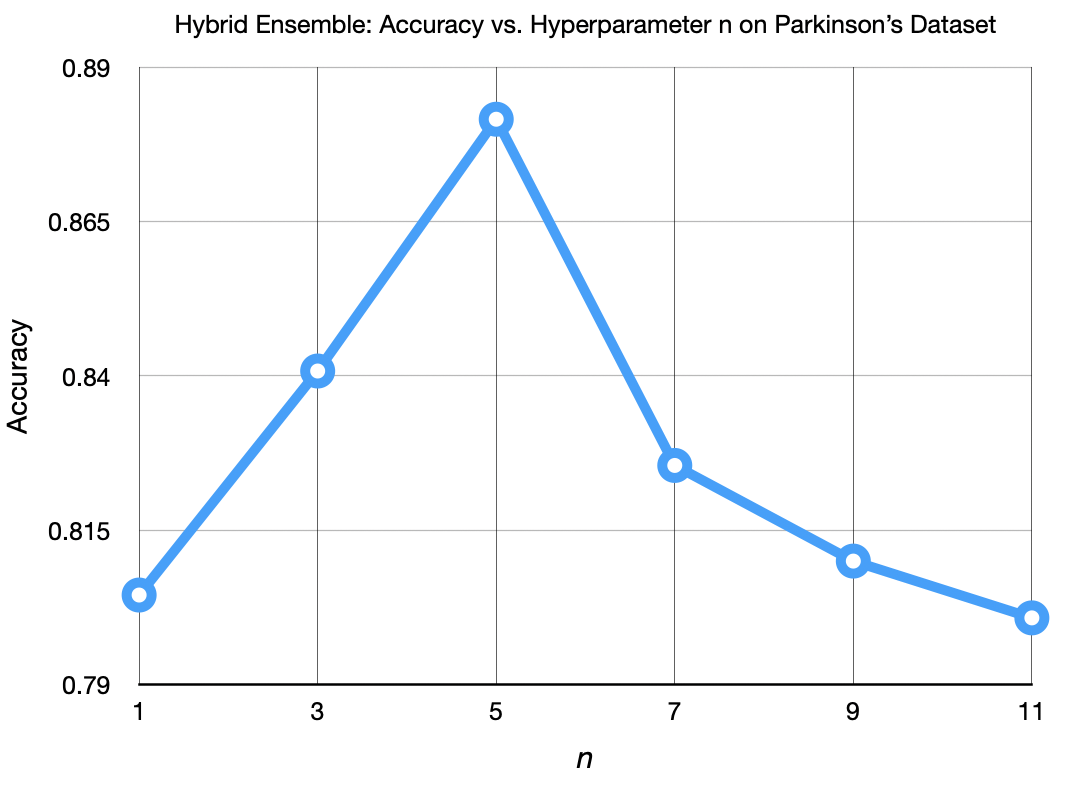
\includegraphics[width=0.6\textwidth]{figures/hybrid_parkinsons_acc.png}
    \caption{Learning Curve on Parkinson's Dataset: Accuracy vs. Hyperparameter $n$}
\end{figure}

\begin{figure}[H]
    \centering
    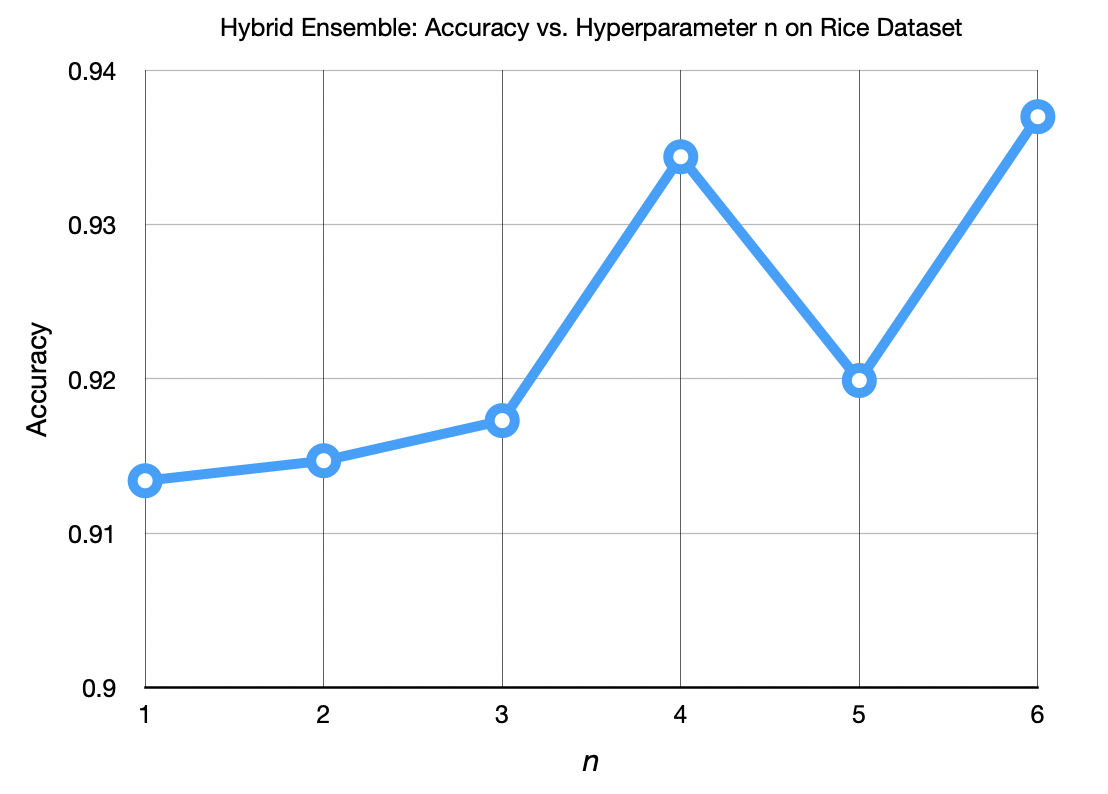
\includegraphics[width=0.6\textwidth]{figures/hybrid_rice_acc.png}
    \caption{Learning Curve on Parkinson's Dataset: Accuracy vs. Hyperparameter $n$}
\end{figure}

\noindent \textbf{Analysis and Interpretation:}

\noindent We can see in the performance on both datasets that the accuracy increases as $n$ increases to 4 or 5.
This is because the variance from bootstrapping along with ensembling voting is allowing the algorithm to reach better conclusions. 
However, if we keep increasing $n$, the number of bootstrapped datasets increases to a point where accuracy begins decreasing.
This is due to the fact that the variance from bootstrapping begins leading to innacuracy on the kNN datasets, and thus drags our accuracy down.

\newpage


\subsection{Overall Results Summary}

The table below summarizes the best performance achieved by each algorithm on the datasets.

\begin{table}[H]
\centering
\resizebox{\textwidth}{!}{%
\begin{tabular}{|l|c|c|c|c|c|c|c|c|c|c|}
\hline
 & \multicolumn{2}{c|}{\textbf{Dataset 1}} & \multicolumn{2}{c|}{\textbf{Dataset 2}} & \multicolumn{2}{c|}{\textbf{Dataset 3}} & \multicolumn{2}{c|}{\textbf{Dataset 4}} & \multicolumn{2}{c|}{\textbf{Dataset 5}} \\ \hline
 & \textbf{Accuracy} & \textbf{F1-Score} & \textbf{Accuracy} & \textbf{F1-Score} & \textbf{Accuracy} & \textbf{F1-Score} & \textbf{Accuracy} & \textbf{F1-Score} & \textbf{Accuracy} & \textbf{F1-Score} \\ \hline
\textbf{k-NN} & \cellcolor[HTML]{C0C0C0}0.9894 & \cellcolor[HTML]{C0C0C0}0.9894 & & & & & & & & \\ \hline
\textbf{Decision Tree} & & & & & & & 0.8637 & 0.8636 & 0.5020 & 0.4985 \\ \hline
\textbf{Random Forest} & 0.9722 & 0.9721 & & & & & 0.8591 & 0.8591 & 0.7020 & 0.6957 \\ \hline
\textbf{Neural Network} & 0.9750 & 0.9749 & & & & & \cellcolor[HTML]{C0C0C0}0.8652 & \cellcolor[HTML]{C0C0C0}0.8652 & \cellcolor[HTML]{C0C0C0}0.7440 & \cellcolor[HTML]{C0C0C0}0.7410 \\ \hline
\textbf{kNN-DT Ensemble} & & & 0.8816 & 0.8607 & 0.9370 & 0.9370 & & & & \\ \hline
\end{tabular}%
}
\caption{Overall Performance Summary Table}
\end{table}





\end{document}